\begin{thebibliography}{0}
  \bibitem{anleitung} F95-Versuchsanleitung Version 1.5
\end{thebibliography}

\section{Appendix}
\begin{figure}[h]
  \caption{Überlagerung bei verschiedenen Translationen der Kamera}
  \label{pic:transl}
  \begin{subfigure}{0.48\linewidth}
    \centering
    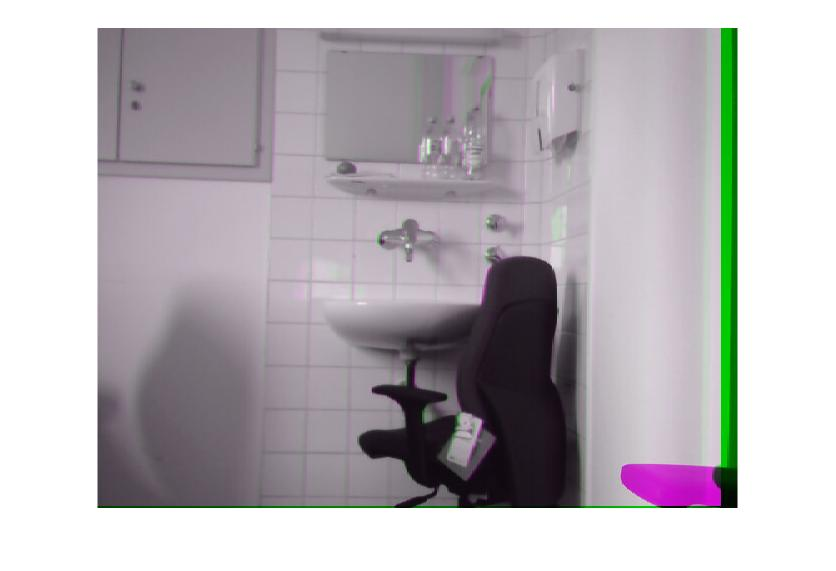
\includegraphics[width=\linewidth]{images/A1_05cm.jpg}
    \vspace{-30pt}
    \caption{\SI{5}{\centi\meter}}
  \end{subfigure}
  \hfill
  \begin{subfigure}{0.48\linewidth}
    \centering
    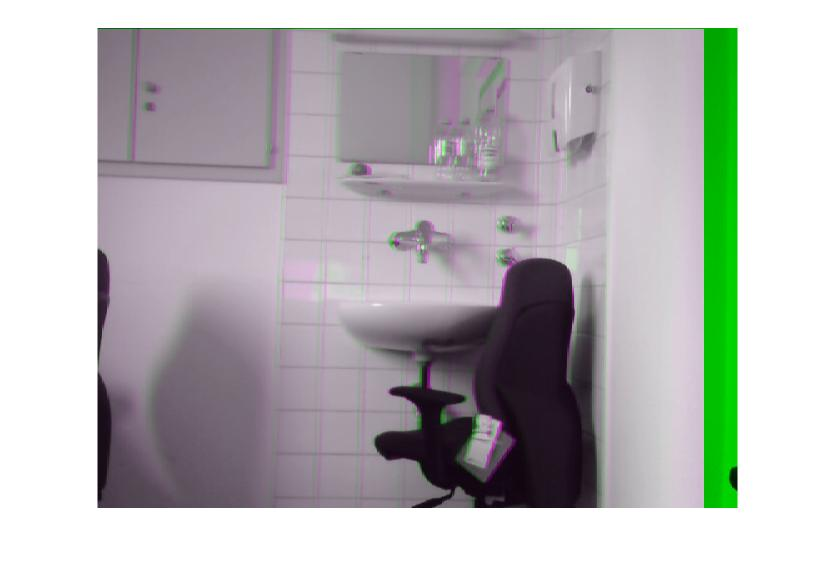
\includegraphics[width=\linewidth]{images/A1_10cm.jpg}
    \vspace{-30pt}
    \caption{\SI{10}{\centi\meter}}
  \end{subfigure}
  \vfill
  \begin{subfigure}{0.48\linewidth}
    \centering
    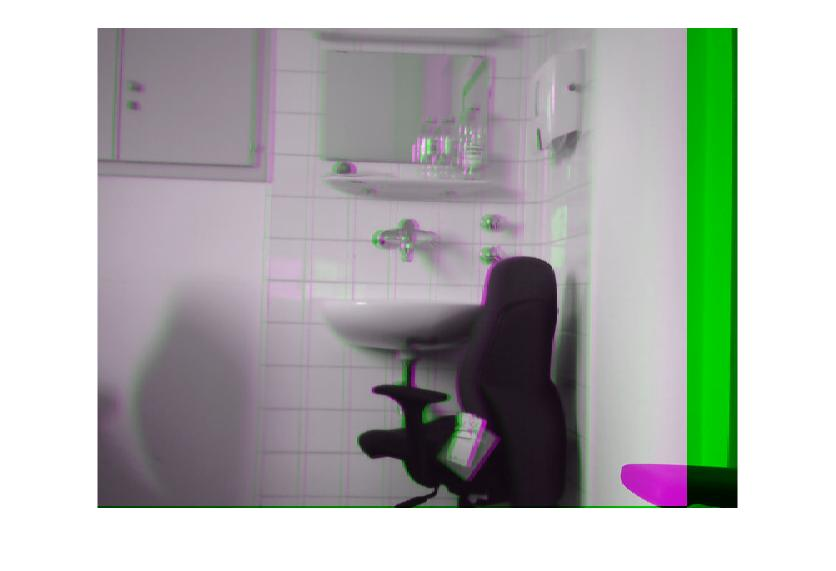
\includegraphics[width=\linewidth]{images/A1_15cm.jpg}
    \vspace{-30pt}
    \caption{\SI{15}{\centi\meter}}
  \end{subfigure}
  \hfill
  \begin{subfigure}{0.48\linewidth}
    \centering
    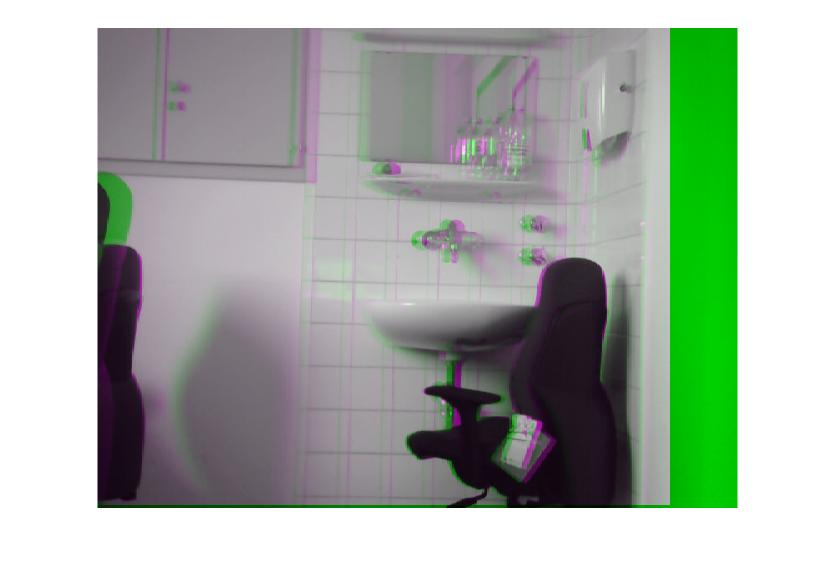
\includegraphics[width=\linewidth]{images/A1_20cm.jpg}
    \vspace{-30pt}
    \caption{\SI{20}{\centi\meter}}
  \end{subfigure}
  \vfill
  \begin{subfigure}{0.48\linewidth}
    \centering
    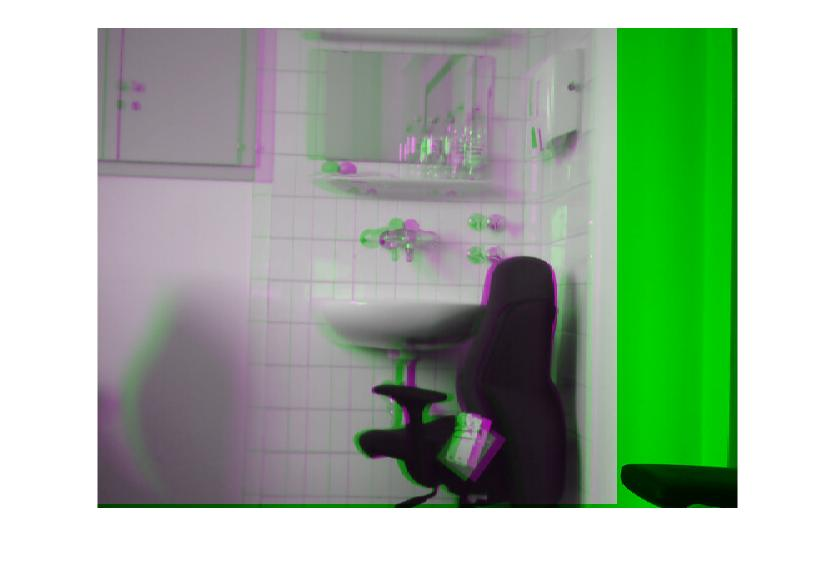
\includegraphics[width=\linewidth]{images/A1_35cm.jpg}
    \vspace{-30pt}
    \caption{\SI{35}{\centi\meter}}
  \end{subfigure}
  \hfill
  \begin{subfigure}{0.48\linewidth}
    \centering
    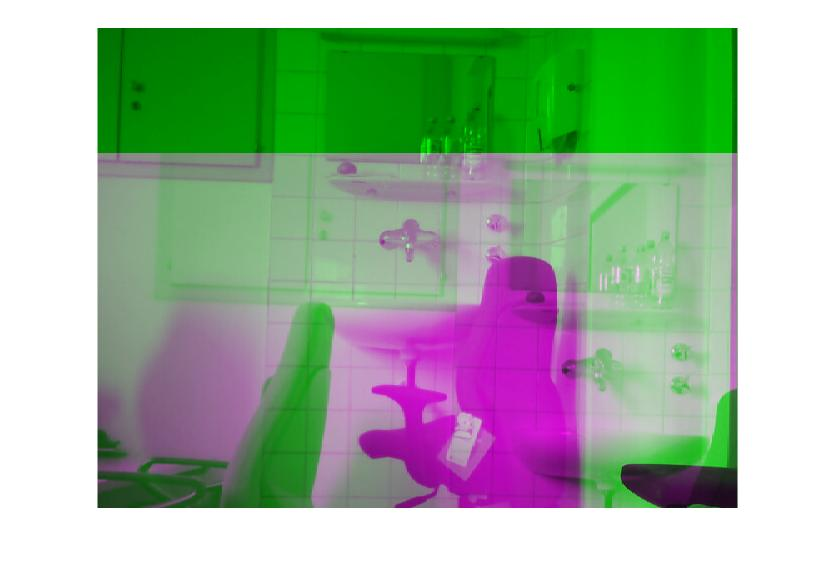
\includegraphics[width=\linewidth]{images/A1_65cm.jpg}
    \vspace{-30pt}
    \caption{\SI{65}{\centi\meter}}
  \end{subfigure}
\end{figure}
\newpage
\begin{figure}[ht]
  \caption{Qualitätsunterschiede bei verschiedenen Registrierungsstrategien}
  \label{pic:A3}
  \begin{subfigure}{\linewidth}
    \centering
    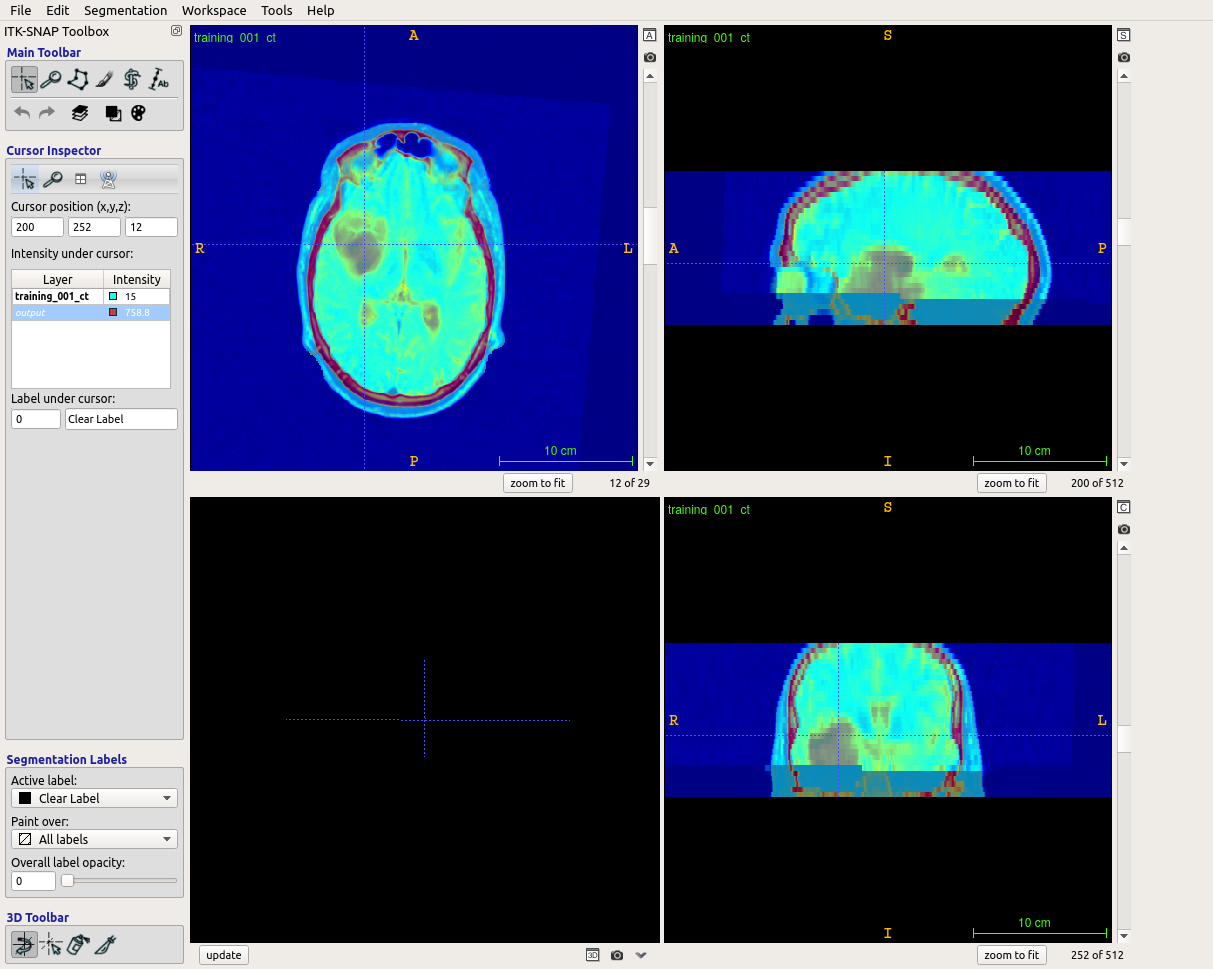
\includegraphics[height=0.44\textheight]{images/A3_good.png}
    \caption{Gute Überlagerung}
  \end{subfigure}
  \vfill
  \begin{subfigure}{\linewidth}
    \centering
    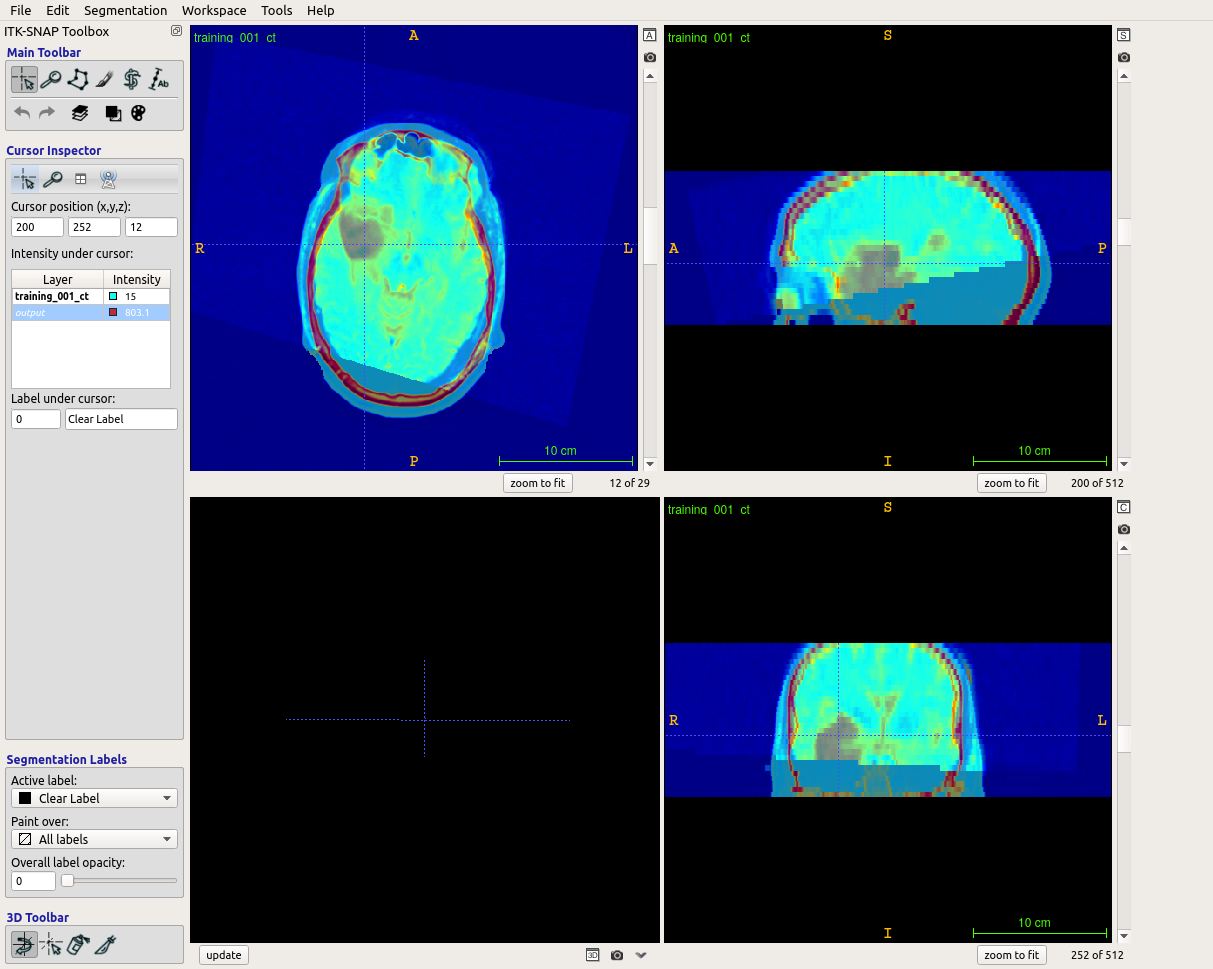
\includegraphics[height=0.44\textheight]{images/A3_bad.png}
    \caption{Schlechte Überlagerung}
  \end{subfigure}
\end{figure}
\newpage
\begin{figure}[ht]
  \caption{Bilder der deformierbaren Registrierung}
  \label{pic:deform}
  \begin{subfigure}{0.32\linewidth}
    \centering
    
\includegraphics[width=\linewidth]{images/A4_5gppd.png}
    \caption{\SI{5}{gppd}}
  \end{subfigure}
  \hfill
  \begin{subfigure}{0.32\linewidth}
    \centering
    
\includegraphics[width=\linewidth]{images/A4_10gppd.png}
    \caption{\SI{10}{gppd}}
  \end{subfigure}
  \hfill
  \begin{subfigure}{0.32\linewidth}
    \centering
    
\includegraphics[width=\linewidth]{images/A4_20gppd.png}
    \caption{\SI{20}{gppd}}
  \end{subfigure}
  \vfill
  \begin{subfigure}{0.32\linewidth}
    \centering
    
\includegraphics[width=\linewidth]{images/A4_30gppd.png}
    \caption{\SI{30}{gppd}}
  \end{subfigure}
  \hfill
  \begin{subfigure}{0.32\linewidth}
    \centering
    
\includegraphics[width=\linewidth]{images/A4_50gppd.png}
    \caption{\SI{50}{gppd}}
  \end{subfigure}
  \hfill
  \begin{subfigure}{0.32\linewidth}
    \centering
    
\includegraphics[width=\linewidth]{images/A4_100gppd.png}
    \caption{\SI{100}{gppd}}
  \end{subfigure}
  \vfill
  \begin{subfigure}{0.32\linewidth}
    \centering
    
\includegraphics[width=\linewidth]{images/A4_fixed.png}
    \caption{Zielbild}
  \end{subfigure}
  \hfill
  \begin{subfigure}{0.32\linewidth}
    \centering
    
\includegraphics[width=\linewidth]{images/A4_moving.png}
    \caption{bewegtes Bild}
  \end{subfigure}
  \hfill
  \begin{subfigure}{0.32\linewidth}
    \centering
    
\includegraphics[width=\linewidth]{images/A4_checkerboard.png}
    \caption{Schachbrett}
  \end{subfigure}
\end{figure}
\clearpage
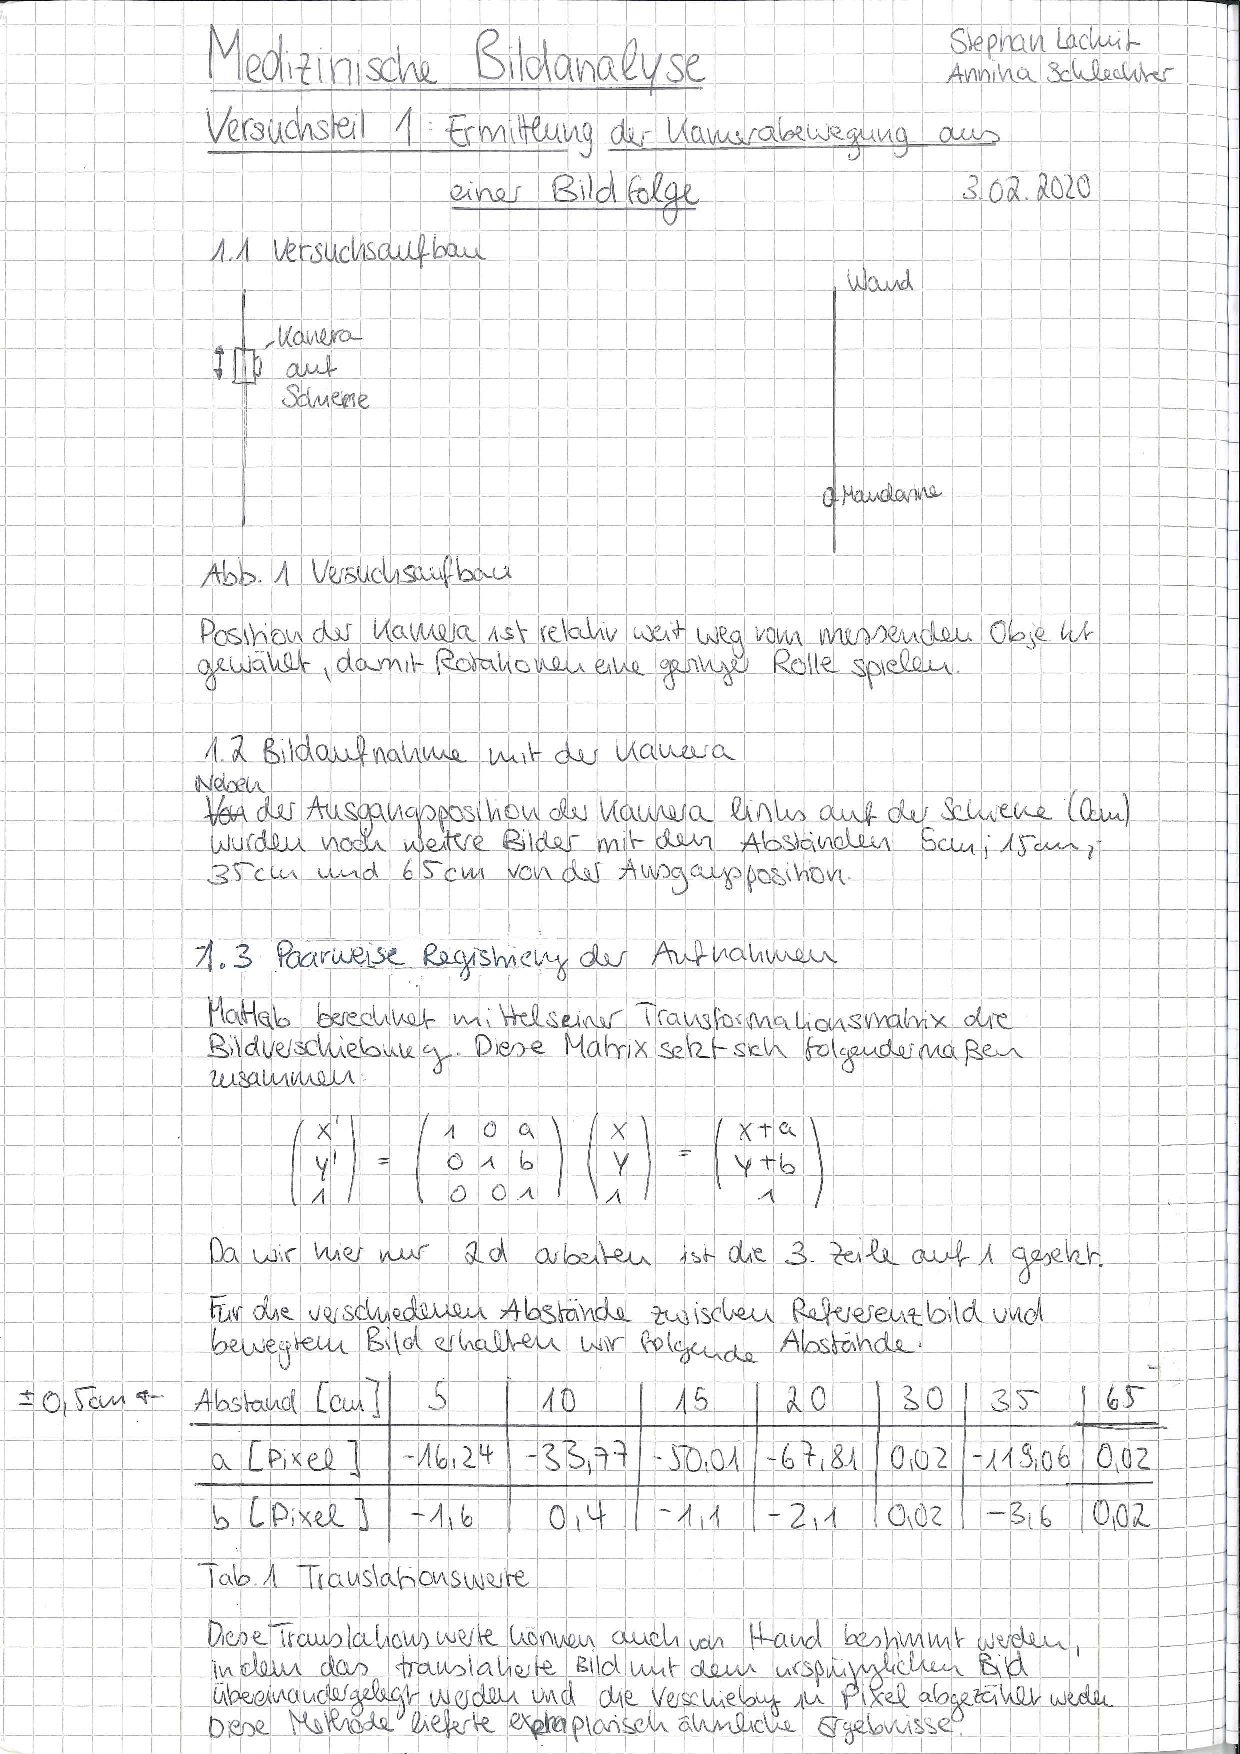
\includepdf[offset=10mm -12mm]{images/protokoll1.pdf}
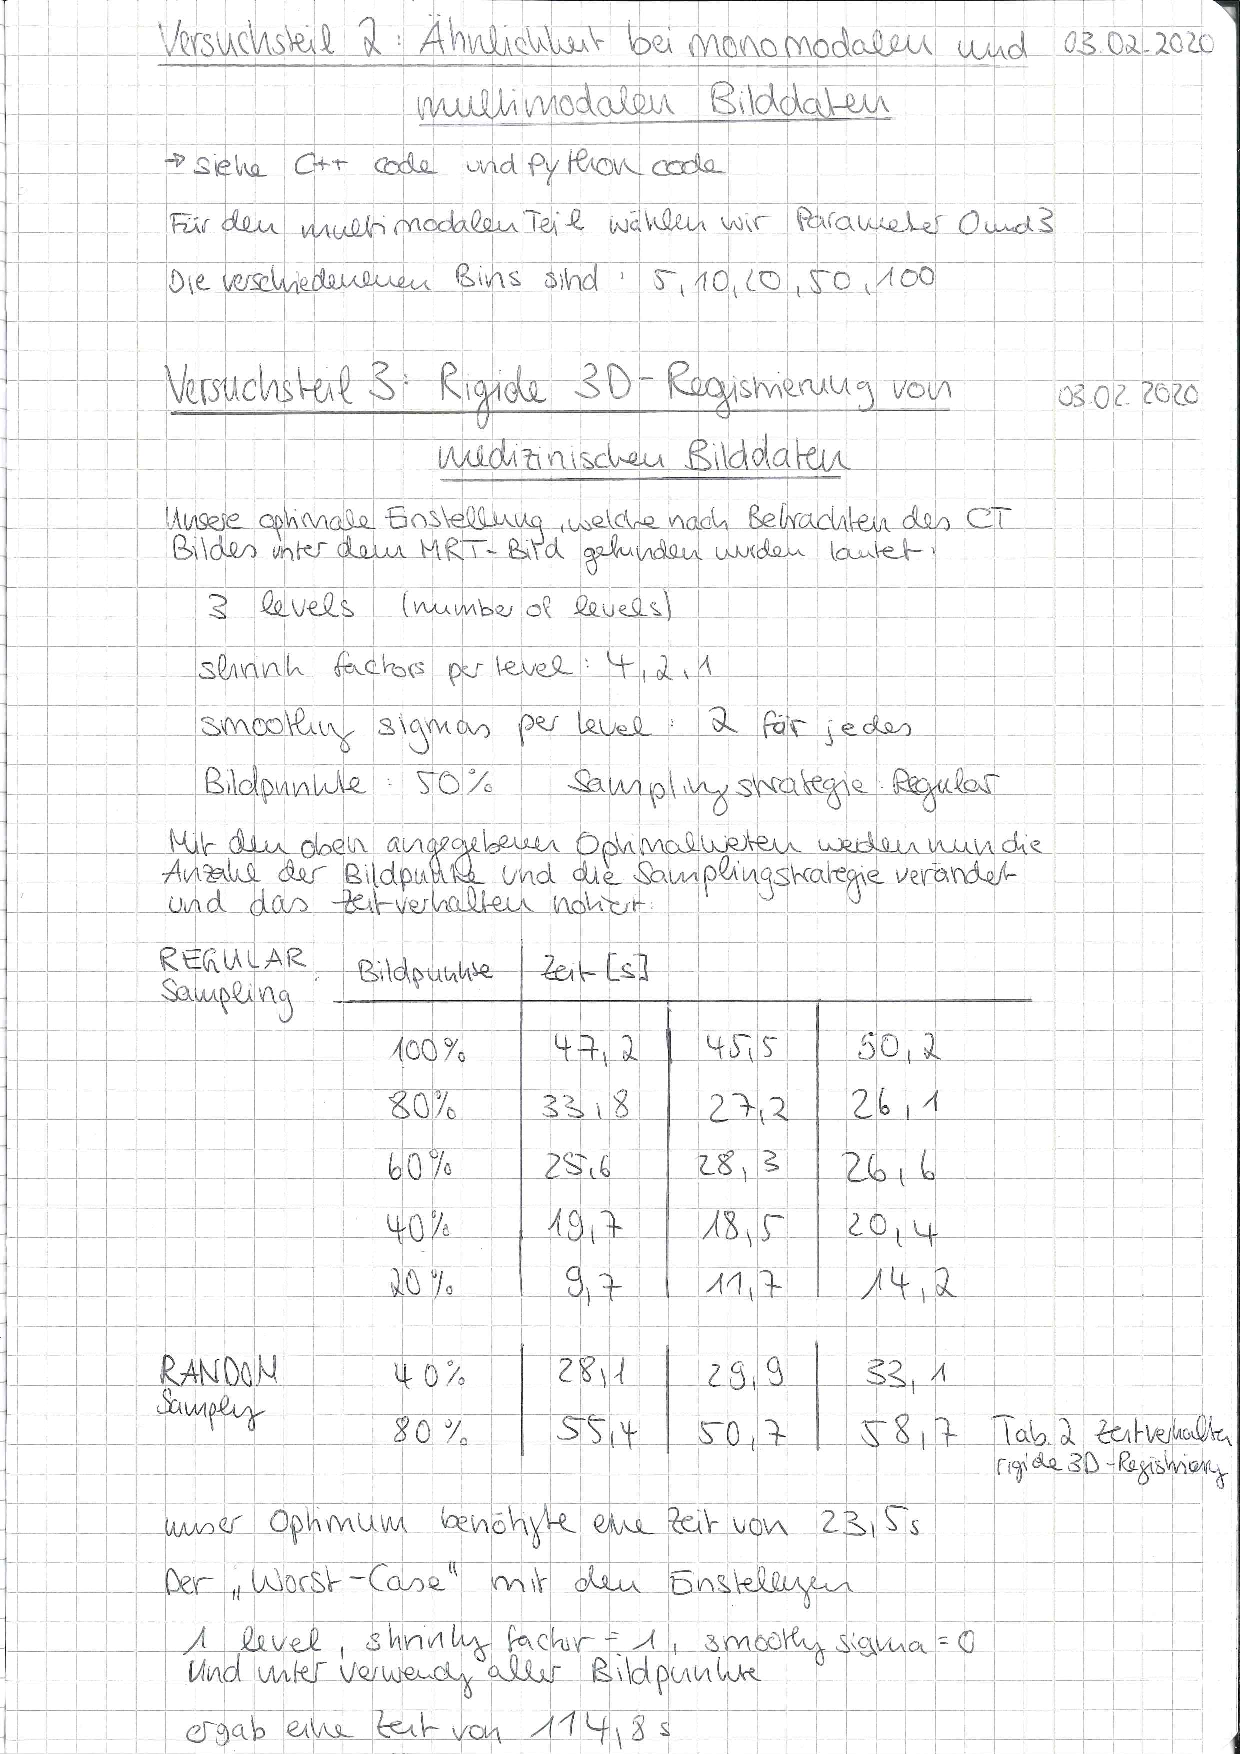
\includepdf[offset=10mm -12mm]{images/protokoll2.pdf}
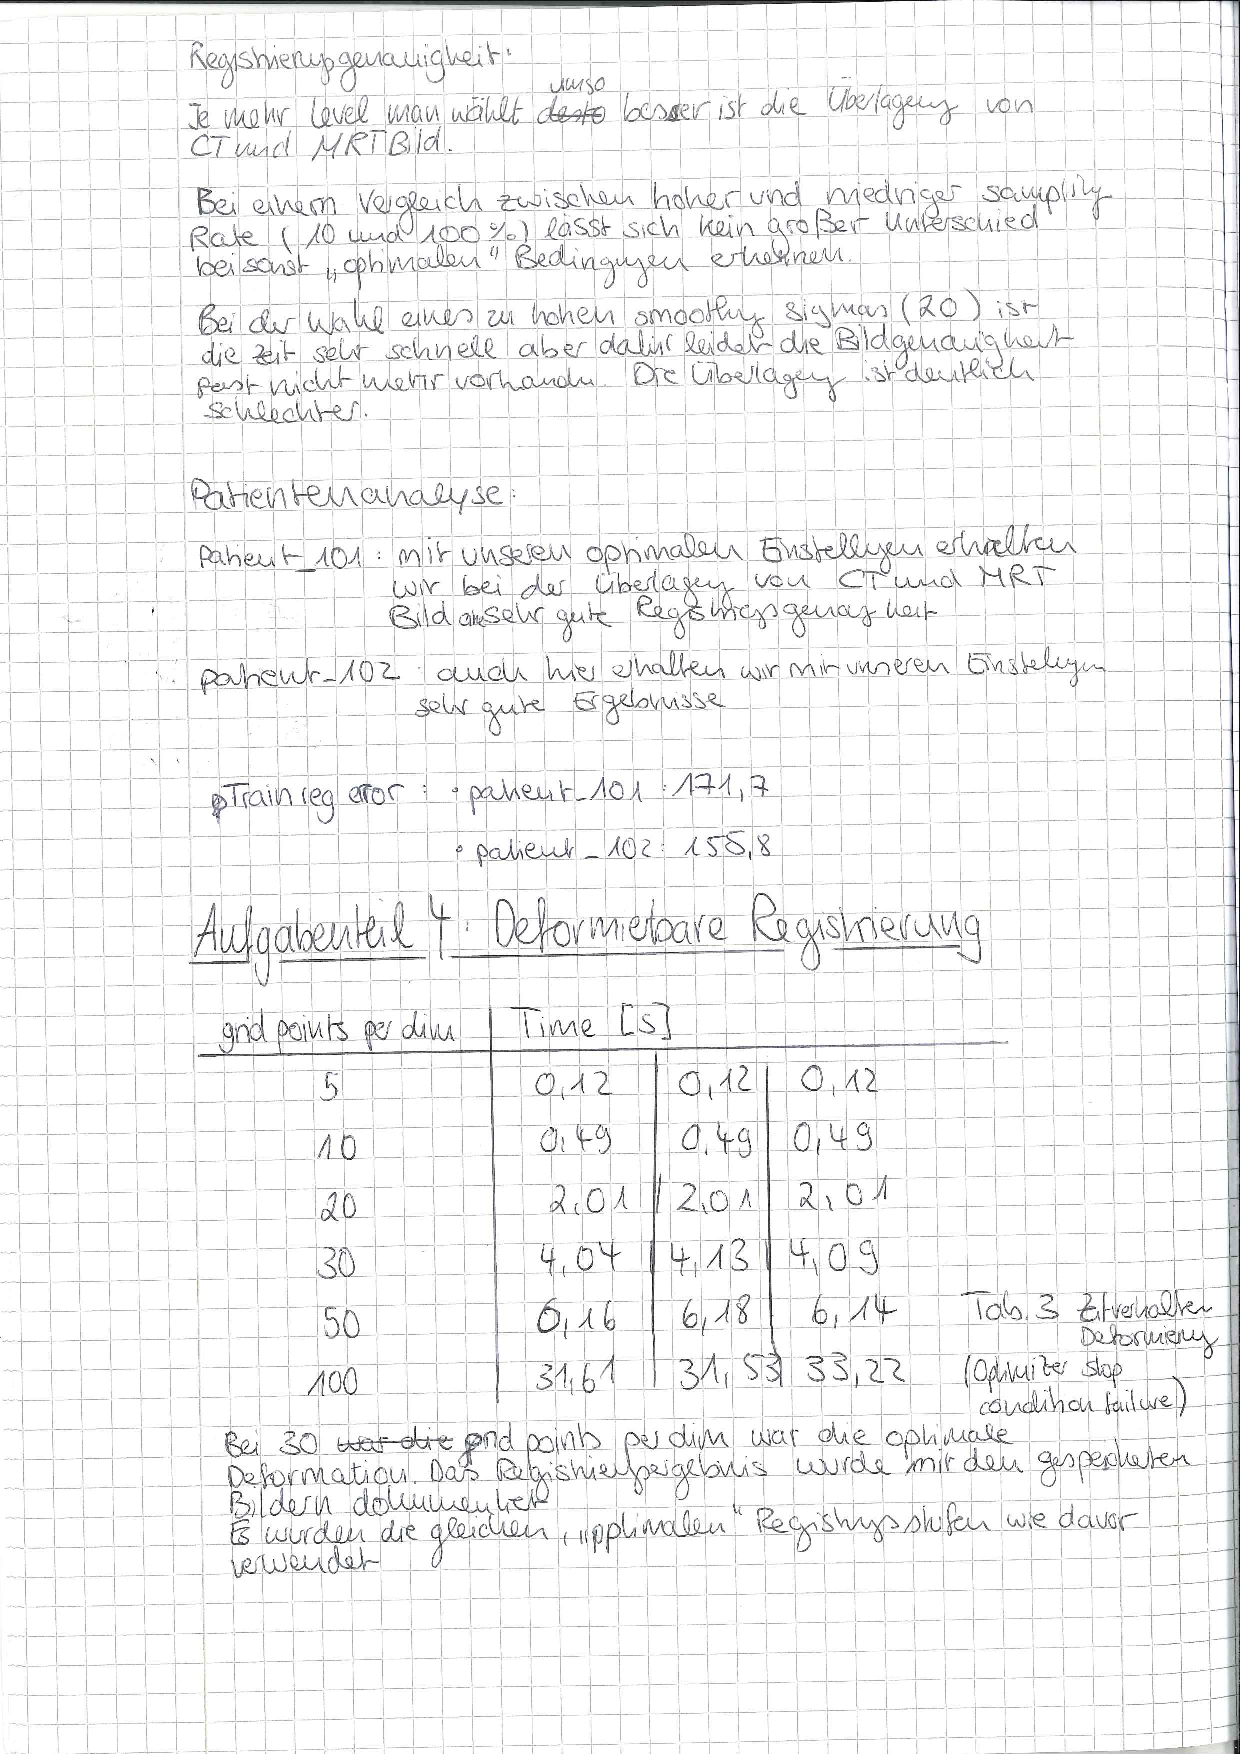
\includepdf[offset=10mm -12mm]{images/protokoll3.pdf}
